
{\setbeamertemplate{footline}{}
\begin{frame}[noframenumbering]
		\titlepage
\end{frame}
}

\begin{frame}	
	\begin{figure}[h!]
		\centering
		\begin{subfigure}[b]{0.4\linewidth}
			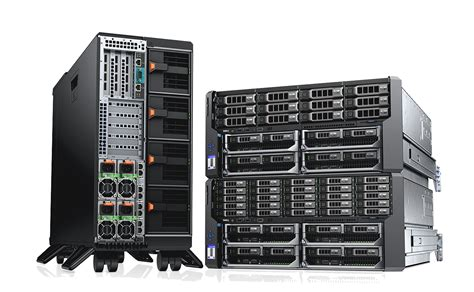
\includegraphics[width=\linewidth]{images/server.jpg}
			\caption{Серверы.}
		\end{subfigure}
		\hfill
		\begin{subfigure}[b]{0.4\linewidth}
			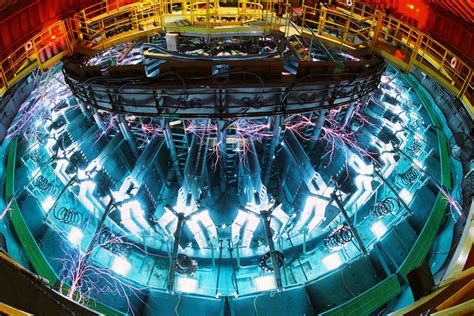
\includegraphics[width=\linewidth]{images/accelerator.jpg}
			\caption{Ускорители.}
		\end{subfigure}
	\end{figure}
	\par
	Существует множество задач, в которых необходимо обрабатывать много независимых событий.
\end{frame}


\begin{frame}{Сопрограммы}
	\begin{itemize}
		\item \textbf{Сопрограмма} (англ. coroutine) - программный модуль, организованный для обеспечения взаимодействия с другими модулями по принципу кооперативной многозадачности.
		
		\item Сопрограммы способны приостанавливать свое выполнение, сохраняя \textit{контекст} 
		(программный стек и регистры), и передавать управление другой.
	\end{itemize}
\end{frame}

\begin{frame}{Ключевые отличия от потоков ОС}
	\begin{itemize}
		\item Переключение контекста сопрограммы требует меньше накладных расходов, чем потока.
		\item Как правило меньший размер стека, а значит, потребление памяти так же меньше.
	\end{itemize}
\end{frame}

\begin{frame}{Поддержка в языках программирования}
	\begin{figure}
	\centering
	\hfill
	\begin{subfigure}[b]{0.22\linewidth}
		
\includegraphics[width=\linewidth]{images/cpp.png}
		\caption{С++20}
	\end{subfigure}
	\hfill
	\begin{subfigure}[b]{0.25\linewidth}
		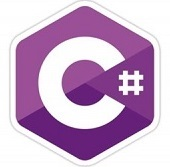
\includegraphics[width=\linewidth]{images/csharp.jpg} 
		\caption{С\#}
	\end{subfigure}
	\hfill
	\begin{subfigure}[b]{0.27\linewidth}
		
\includegraphics[width=\linewidth]{images/go.jpg}
		\caption{Go}
	\end{subfigure}
	
	\end{figure}
	\par
	В языке Java сопрограммы не реализованы.
\end{frame}

\begin{frame}
	
\includegraphics[scale=0.5]{images/loom.jpg}
	\begin{itemize}
		\item Project Loom – проект на базе OpenJDK, целью которого является разработка сопрограмм для языка Java. 
		\item На данный момент уже доступна ранняя версия проекта.
	\end{itemize}
\end{frame}

\begin{frame}{Цели и задачи}
	Цель: реализация прототипа сопрограмм в Java.
	\par
	Поставленные задачи:
	\begin{itemize}
		\item Разработать тесты для сравнения производительности потоков и сопрограмм.
		\item Реализовать переключение сопрограмм.
		\item Реализовать трассировку ссылок объектов на стеках сопрограмм для сборки мусора.
		\item Сравнить производительность сопрограмм и потоков. 
	\end{itemize}
	Работа проводится на базе Huawei JDK.
\end{frame}

\begin{frame}{Тесты производительности}
	Был создан набор тестов производительности сопрограмм для языков Go, Java (с “Loom Project”).
	
	Тесты создавались для измерения 2 параметров.
	\begin{itemize}
		\item Скорость переключения контекста.
		\item Потребление памяти.
	\end{itemize}
	Репозиторий с тестами: https://github.com/minium2/coroutines-benchmark
\end{frame}

\begin{frame}{Переключение сопрограмм}
	\begin{figure}
		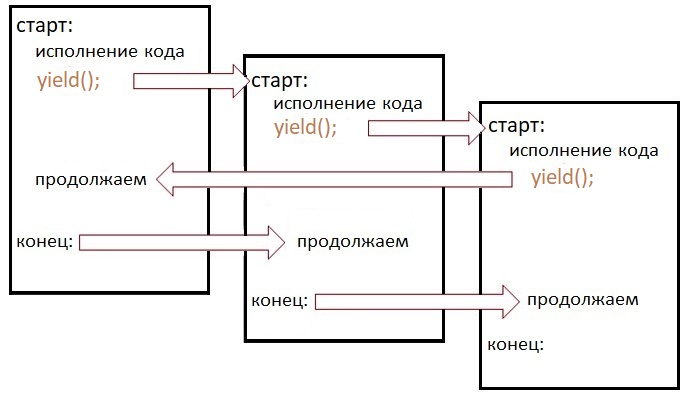
\includegraphics[scale=0.5]{images/scheme.jpg}
	\end{figure}
	\par
	Подходы к реализации:
	\begin{itemize}
		\item OpenJDK(Проект "Loom"): копирование стека сопрограммы при переключении.
		\item Go и HuaweiJDK: изменение указателя стека.
	\end{itemize}
\end{frame}

\begin{frame}{Трассировка стеков}

	\begin{itemize}
		\item Для работы сборщика мусора необходимо хранить адрес начала и конца стека каждой сопрограммы.
		\item При сборке мусора сканируются все стеки сопрограмм для поиска корневого множества живых объектов.
	\end{itemize}
\end{frame}	

\begin{frame}{Результаты: скорости переключения потоков и сопрограмм}
	Ubuntu, Intel Core i7-8700, 31 Гб ОЗУ, HuaweiJDK
	\par Каждое значение усреднено по 100 измерениям. 
	\par Для измерения используется только одно ядро ЦП.
	\begin{table}[H]
		%\caption{Число переключений корутин}\label{inc-matrix}
		\begin{tabular}{|c|c|c|c|c|c|}
			\hline \multirow{2}{*}{Шт.} & \multicolumn{2}{|c|}{Число переключений, 1/сек.}    \\
			\cline{2-3}    & Сопрограммы              & Потоки                    \\
			\hline 100     & 1'246'756 $\pm$ 12'961 & 2'306'346 $\pm$ 49'831  \\
			\hline 1'000   & 1'199'142 $\pm$ 11'803 & 2'300'279 $\pm$ 27'180  \\
			\hline 5'000   & 1'075'559 $\pm$ 59'328 & 1'553'872 $\pm$ 36'832  \\
			\hline 10'000  & 1'016'802 $\pm$ 9'990  & 1'015'976 $\pm$ 29'096  \\ 
			\hline 20'000  & 916'809 $\pm$ 8'354    & 753'123 $\pm$ 28'248    \\ 
			\hline 30'000  & 858'994 $\pm$ 4'307    & 555'720 $\pm$ 16'102    \\ 
			\hline 40'000  & 790'015 $\pm$ 8'033    & 436'529 $\pm$ 12'334    \\ 
			\hline 50'000  & 756'523 $\pm$ 8'232    & 361'088 $\pm$ 7'853     \\ 
			\hline 
		\end{tabular}
	\end{table}
	
\end{frame}


\begin{frame}{Результаты: скорости переключения сопрограмм в управляемых средах}
	Ubuntu, Intel Core i7-8700, 31 Гб ОЗУ, HuaweiJDK
	\par Каждое значение усреднено по 100 измерениям. 
	
	\begin{table}[H]
		%\caption{Число переключений корутин}\label{inc-matrix}
		\begin{tabular}{|c|c|c|c|c|c|}
			\hline \multirow{2}{*}{Шт.} & \multicolumn{3}{|c|}{Число переключений, 1/сек.}                        \\
			\cline{2-4}     & HuaweiJDK                & OpenJDK("Loom Project")     & Go                         \\
			\hline 100      & 1'246'756 $\pm$ 12'961 & 1'900'009 $\pm$ 19'732    & 18'187'799 $\pm$ 219'367 \\
			\hline 1'000    & 1'199'142 $\pm$ 11'803 & 1'775'239 $\pm$ 20'491    & 17'934'078 $\pm$ 332'778 \\
			\hline 5'000    & 1'075'559 $\pm$ 59'328 & 1'703'631 $\pm$ 30'498    & 12'892'417 $\pm$ 339'410 \\  
			\hline 10'000   & 1'016'802 $\pm$ 9'990  & 1'924'971 $\pm$ 234'982   & 8'307'791 $\pm$ 79'652   \\  
			\hline 20'000   & 916'809 $\pm$ 8'354    & 1'863'342 $\pm$ 217'482   & 7'045'984 $\pm$ 72'584   \\ 
			\hline 30'000   & 858'994 $\pm$ 4'307    & 1'772'720 $\pm$ 182'023   & 6'391'629 $\pm$ 94'370   \\ 
			\hline 40'000   & 790'015 $\pm$ 8'033    & 1'606'534 $\pm$ 194'728 	 & 5'790'831 $\pm$ 66'910	  \\ 
			\hline 50'000   & 756'523 $\pm$ 8'232    & 1'503'444 $\pm$ 157'186   & 5'292'780 $\pm$ 121'844  \\  
			\hline 
		\end{tabular}
	\end{table}	
\end{frame}


\begin{frame}{Результаты: потребление памяти}
	Ubuntu, Intel Core i7-8700, 31 Гб ОЗУ
	\begin{table}[H]
		\begin{tabular}{|c|c|c|c|c|c|}
			\hline \multirow{2}{*}{Шт.} & \multicolumn{3}{|c|}{Резидентная память}  \\
			\cline{2-4}    & HuaweiJDK   & OpenJDK    & Go       \\
			\hline 100     & 18 Mб       & 130 Mб     & 3040 Kб  \\
			\hline 1000    & 23 Mб       & 161 Mб     & 3105 Kб  \\
			\hline 5000    & 30 Mб       & 187 Mб     & 3156 Kб  \\
			\hline 10000   & 35 Mб       & 193 Mб     & 3308 Kб  \\
			\hline 20000   & 40 Mб       & 196 Mб     & 3320 Kб  \\
			\hline 30000   & 45 Mб       & 197 Mб     & 3350 Kб  \\
			\hline 40000   & 49 Mб       & 200 Mб     & 3390 Kб  \\
			\hline 50000   & 55 Mб       & 202 Mб     & 3407 Kб  \\ 
			\hline 
		\end{tabular}
	\end{table}
\end{frame}

\begin{frame}{Результаты: потребление памяти}
	Ubuntu, Intel Core i7-8700, 31 Гб ОЗУ, HuaweiJDK
	\begin{table}[H]
		%\caption{Число переключений корутин}\label{inc-matrix}
		\begin{tabular}{|c|c|c|c|c|c|}
			\hline \multirow{2}{*}{Шт.} & \multicolumn{2}{|c|}{Размер физической памяти}  \\
			\cline{2-3}    & Сопрограммы   & Потоки    \\
			\hline 100     & 18 Mб         & 34 Mб     \\
			\hline 1000    & 23 Mб         & 35 Mб     \\
			\hline 5000    & 30 Mб         & 37 Mб     \\
			\hline 10000   & 35 Mб         & 40 Mб     \\
			\hline 20000   & 40 Mб         & 49 Mб     \\
			\hline 30000   & 45 Mб         & 56 Mб     \\
			\hline 40000   & 49 Mб         & 63 Mб     \\
			\hline 50000   & 55 Mб         & 72 Mб     \\ 
			\hline 
		\end{tabular}
	\end{table}
\end{frame}

\begin{frame}{План дальнейших работ} 
	\begin{itemize}
		\item Реализовать функцию переключения контекста.
		\item Поддержка synchronized блоков.
		\item Переключение сопрограммы при вызове ввода вывода.
	\end{itemize}
\end{frame}

\begin{frame}{Выводы}
	\begin{itemize}
		\item Создан набор тестов для сравнения производительности потоков и сопрограмм.
		\item Реализовано переключение контекста сопрограмм.
		\item Разработана трассировка ссылок объектов на стеках сопрограмм.
		\item Проведено сравнение результаты тестов производительности.
	\end{itemize}
\end{frame}

